\documentclass[professionalfont]{beamer}
\usetheme[secheader]{Madrid}

\usepackage{amssymb, amsmath, mathrsfs}
\usepackage{amsthm}
\usepackage{subfig}
\usepackage{animate}
\usepackage{newtxtext,newtxmath}

\theoremstyle{remark}
\newtheorem{remark}[theorem]{Remark}

\newcommand{\abs}[1]{\lvert#1\rvert}
\newcommand{\norm}[1]{\lVert#1\rVert}
\DeclareMathOperator{\re}{Re}
\DeclareMathOperator{\im}{Im}
\newcommand{\ud}{\mathrm{d}}
\newcommand{\e}{\mathrm{e}}
\renewcommand{\i}{\mathrm{i}}

\AtBeginSection[]{
  \begin{frame}
  \vfill
  \centering
  \begin{beamercolorbox}[sep=8pt,center,shadow=true,rounded=true]{title}
    \usebeamerfont{title}\insertsectionhead\par%
  \end{beamercolorbox}
  \vfill
  \end{frame}
}
	
\title{Comparison of Continuum and Atomistic Models for Chemical Diffusion and Phase Separation}
\date{July 2, 2024}
\author{Isaac Viviano}

\begin{document}

\begin{frame}

	\maketitle

\end{frame}

\begin{frame}{Outline}
	
	\tableofcontents

\end{frame}

\section{Motivation}

\begin{frame}{Motivation}
	
	For any model, interesting to ask which approximations are worth making

	\vspace{10 pt}

	Chemical modeling considerations:
	\begin{itemize}
		\item Physical reality is quantization
		\item Quantum modeling is extremely expensive
		\item Classical particle-based models more feasible
		\item Often interested in bulk properties
		\item Sufficiently large systems of classical particles are still expensive
		\item When is the continuum limit a reasonable model?
	\end{itemize}

	
\end{frame}

\section{Chemical Processes}

\begin{frame}{Diffusion} % REMOVE EQUATION NUMBERS

	Spontaneous reduction in a chemical concentration gradient over time

	\begin{figure} % larger and caption
		\centering 
		\subfloat[\centering Continuum]{{\animategraphics[width = 5cm, every = 1, loop, autoplay]{6}{media/continuum_diff/cont_diff-}{0}{99}} }
		\qquad
		\subfloat[\centering Atomistic]{{\animategraphics[width = 4.5cm, every = 1, loop, autoplay]{6}{media/particle_diff/part_diff-}{0}{99}}}
	\end{figure} 
	
\end{frame}

\begin{frame}{Phase Separation} % IMAGE STICKING OFF THE SIDE

	\begin{columns}
		\begin{column}{.55\paperwidth}
			
		\begin{itemize}
			\item Spontaneous separation of a two-component mixture into its constituents
			\item Let $[A],[B]$ be the component concentration functions. Generally, 
			\begin{align*}
				0\le [A],[B]\le1\\
				[A]+[B]=1
			\end{align*}
			\item Order parameter:
			\begin{equation*}
				u:=[A]-[B]=1-2[B]
			\end{equation*}
			\item Spinodal decomposition model (as opposed to chance nucleation)
		\end{itemize}

		\end{column}

		\begin{column}{.45\paperwidth}
			

		\begin{figure}
			% 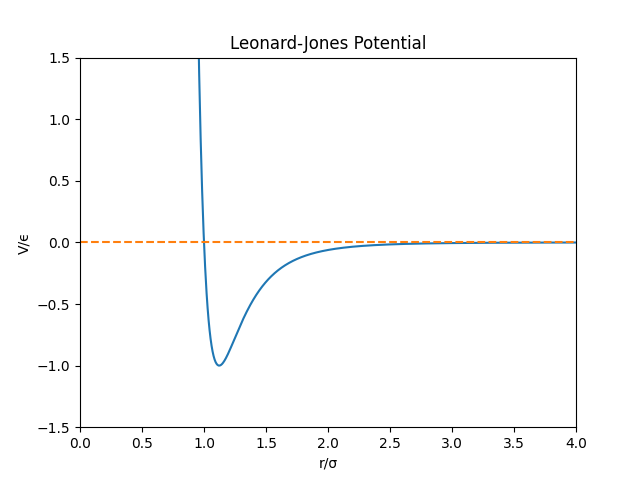
\includegraphics{media/lj_pot.png}
			\animategraphics[width = .45\paperwidth, every = 1, loop, autoplay]{5}{media/AC_sep/AC_sep-}{0}{140}
		\end{figure}

		\end{column}

	\end{columns}
\end{frame}

\section{Model Differences}

\begin{frame}{Modeling Approaches}

	Atomistic Model: Molecular Dynamics
	\begin{itemize}
		\item Collection of discrete classical particles
		\item Approximate interparticle forces simulate Hamiltonian dynamics
		\item Generates time-discretized trajectory of each particle
	\end{itemize}

	Continuum Model: Differential Equations
	\begin{itemize} % WE CONSIDER THREE DIFFERENTIAL EQUATIONS
		\item Order parameter, $u(x,t)$, is a continuous quantity: \begin{equation*}
			u\colon \Omega\times(0,\infty)\to[-1,1],\quad u\in\mathcal{C}^2
		\end{equation*}
		\item Order parameter satisfies a differential equation based on physical laws and modeling assumptions
		\item Numerical method generates time- and space-discretized approximation of $u$
	\end{itemize}

\end{frame}

\begin{frame}{Model Type Comparison}

	Estimate distribution of particles at each MD timestep:
	\begin{itemize}
		\item Choose a resolution to divide the spatial domain into bins
		\item Count the number of atoms in each bin
	\end{itemize}

	\begin{columns}

		\begin{column}{.42\paperwidth}
			
			\centering
			\begin{figure}
				
				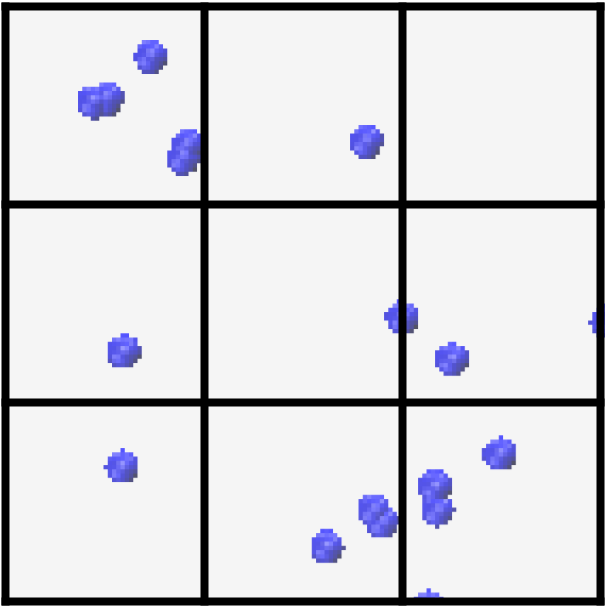
\includegraphics[width = 3 cm]{media/md_bins.png}
			\\ Trajectory Timestep
			\end{figure}
		\end{column}
		
		\begin{column}{.05\paperwidth}

			\centering
			\huge
			\textrightarrow{}
			
		\end{column}

		\begin{column}{.42\paperwidth}
			
			\begin{figure}
				\centering
				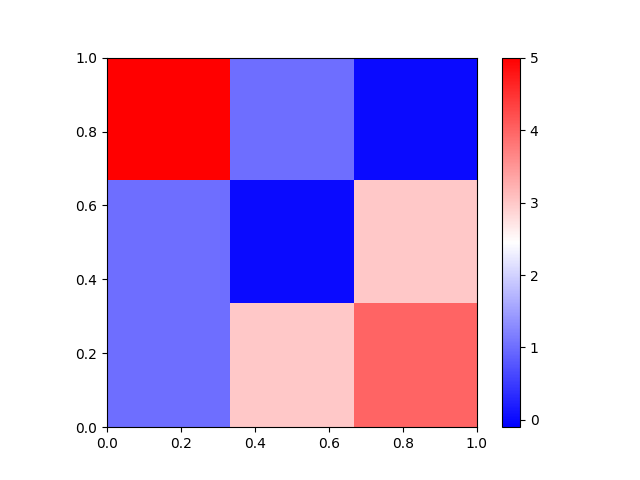
\includegraphics[width = 5 cm]{media/bins.png}
				\\ Order Parameter
			\end{figure}
		\end{column}
	
	\end{columns}
	
\end{frame}

\section{Atomistic Model: Molecular Dynamics}

\begin{frame}{Leonard-Jones Potential}


	Pairwise 6-12 Leonard-Jones potential for internuclear distance $r$:
	\begin{equation}
		V(r)=4\epsilon\left[ \left( \frac{\sigma}{r} \right)^{12}-\left( \frac{\sigma}{r} \right)^6 \right],\quad r<r_c
	\end{equation}
	
	\vspace*{10pt}

	\begin{columns}
		
		\begin{column}{.5\paperwidth}

			\begin{itemize}
				\item Efficient, accurate model for interparticle London Dispersion forces
				\item Parameters $\sigma,\epsilon$ describe equilibrium distance and well depth
				\item Generally implemented with long-range cutoff, $r_c$
			\end{itemize}

			

		\end{column}

		\begin{column}{.4\paperwidth}
			
			\begin{figure}
				\centering
				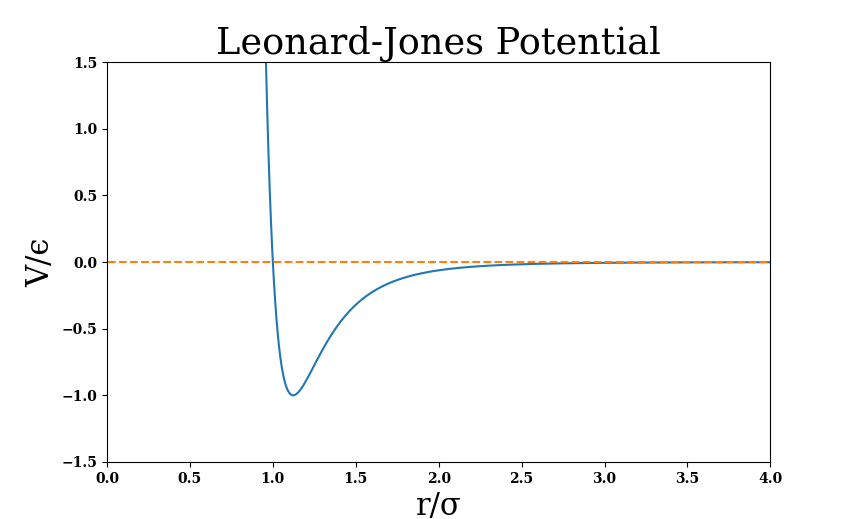
\includegraphics[width = 2in]{media/lg_pot.png}

			\end{figure}
		
		\end{column}

	\end{columns}

	
\end{frame}

\begin{frame}{Leonard-Jones Fluid} 

	Leonard-Jones potential for $N_A$ particles:
	\begin{equation*}
		\mathcal{V}(\mathbf{r})=\sum_{1\le i<j\le N_A}V(r_{ij})
	\end{equation*}
	where $r_{ij}$ is the distance between particles $i$ and $j$.

	\vspace*{10 pt}

	One component:
	\begin{itemize}
		\item Experimentally determined parameters of Argon (noble gas, $Z=18$)
		\item Bulk temperature and pressure match conditions of experiment
		\item Models diffusion of real gas into a vacuum
	\end{itemize}

	\vspace*{10 pt}

	Two component:
	\begin{itemize}
		\item Components $A$ and $B$ present in equal amounts
		\item To trigger phase separation, 
		\begin{equation*}
			\epsilon_{AA}=\epsilon_{BB}>>\epsilon_{AB}\quad\sigma_{AA}=\sigma_{BB}=\sigma_{AB}
		\end{equation*}
	\end{itemize}
	
\end{frame}

\begin{frame}{LAMMPS}

	Large Scale Atomic/Molecular Masively Parallel Simulator - LAMMPS

	\begin{itemize}
		\item Open source code maintainted by national labs
		\item Implements several dynamics integrators
		\item Integrated with various analysis software
		\item User specifies potential $\mathcal{V}$ and initial state
		\item Extract physical/phenomenalogical parameters and state functions from trajectories
		\item MD uniquely allows us to understand how material properties depend on thermodynamic states
	\end{itemize}
	

	\begin{figure}
		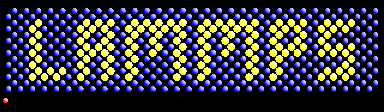
\includegraphics[width = 5cm]{media/lammps.png}
	\end{figure}
	
\end{frame}

\section{Continuum Model: Differential Equations}

\begin{frame}{Gradient Flow}

	Gradient flow of an energy functional $F\colon\mathcal{F}\to\mathbb{R}\cup\{\infty\}$: 
	\begin{equation}
		\frac{\partial u}{\partial t}=-\frac{\partial F}{\partial u}
	\end{equation}
	over a Hilbert space $\mathcal{F}$ with inner product $(\cdot ~, \cdot)_{\mathcal{F}}$.
	\begin{equation*}
		\mathcal{F}=L^2(\Omega)\quad\text{or}\quad\mathcal{F}=H^{-1}(\Omega)
	\end{equation*}
	
	\vspace*{10 pt}
	Energy is nonincreasing in time: 
	\begin{equation*}
		\frac{\ud}{\ud t}F(u)=(\frac{\partial F}{\partial u},\frac{\partial u}{\partial t})_{\mathcal{F}}=(\frac{\partial F}{\partial u},-\frac{\partial F}{\partial u})_{\mathcal{F}}=-\left\|\frac{\partial F}{\partial u}\right\|_{\mathcal{F}}^2\le0
	\end{equation*}

\end{frame}	

	
\begin{frame}{Energy Functionals} 
	
	Diffusion energy functional:
	\begin{equation}
		F_d(u)=\int_\Omega\frac{1}{2}|\nabla u|^2~\ud x
	\end{equation}
	
	Phase energy functional:
	\begin{equation} \label{eq_func}
		F_p(u)=\int_\Omega \left(\psi(u)+\frac{\gamma}{2}|\nabla u|^2\right)~\ud x
	\end{equation}

	\begin{itemize}
		\item Functionals constructed from physical principles
		\item Function spaces chosen so the differential equation satisfies certain physical or mathematical properties
	\end{itemize}
	
\end{frame}

\begin{frame}{Double Well Potential}
	The function $\psi$ in (\ref{eq_func}) is a double-well free energy function:

	\begin{columns}
		\begin{column}{.45\paperwidth}

			\begin{equation*}
				\psi(u):=\frac{1}{4}(u^2-1)^2	
			\end{equation*}

			\begin{figure}
				\centering
				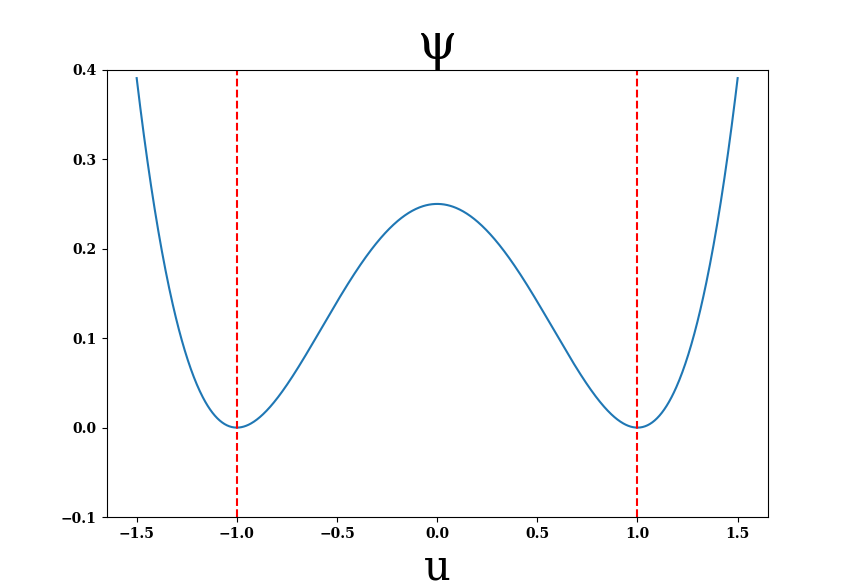
\includegraphics[width = .43\paperwidth]{media/psi.png}
			\end{figure}
			
		\end{column}

		\begin{column}{.45\paperwidth}
			
			\begin{equation*}
				\phi(u):=\psi'(u)=u^3-u
			\end{equation*}

			\begin{figure}
				\centering
				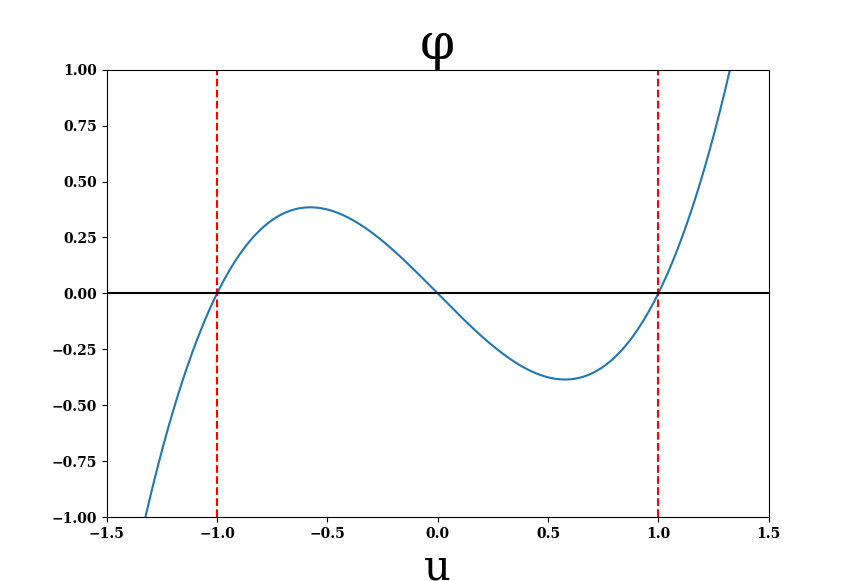
\includegraphics[width = .43\paperwidth]{media/phi.png}
			\end{figure}
			
		\end{column}
	\end{columns}
	% \begin{figure} % SEPARATE
	% 	\begin{center}
	% 		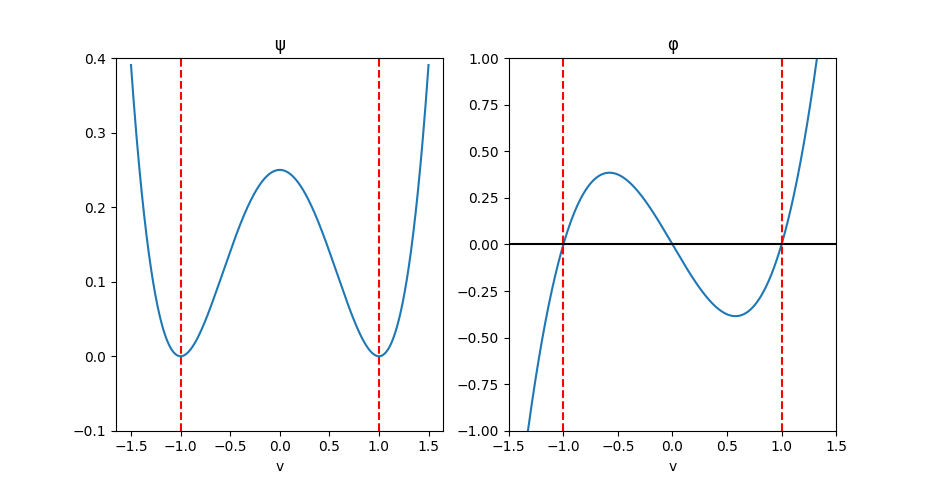
\includegraphics[width = 3in]{media/double_well_pot.png}

			
	% 	\end{center}
	% \end{figure}

	\vspace{5 pt}
	The minima of $\psi$ reflects the stability of pure phases.

\end{frame}

\begin{frame}{Derivation of the Heat Equation}
	For the diffusion energy functional $F_d(u)=\int\frac{1}{2}|\nabla u|^2~\ud x$,
	\begin{align*}
		F_d(u+\epsilon v)&=\int_\Omega\frac{1}{2}|\nabla u+\epsilon \nabla v|^2~\ud x=\frac{1}{2}\|\nabla u+\epsilon\nabla v\|_{L^2}^2\\
		&=\frac{1}{2}\|\nabla u\|^2_{L^2}+\epsilon(\nabla u,\nabla v)_{L^2}+\frac{\epsilon^2}{2}\|\nabla v\|^2_{L^2}\\
		&=F_d(u)+ \epsilon(-\nabla^2u,v)_{L^2}+\epsilon^2F_d(v)
	\end{align*}
	where $(\nabla u,\nabla v)_{L^2}=(-\nabla^2 u,v)_{L^2}$ follows from Green's Identities when $\nabla u$ is periodic. 

	\vspace*{10 pt}

	Therefore, the $L^2$ gradient of the diffusion energy functional satisfies
	\begin{equation*}
		\langle\textcolor{red}{\frac{\partial F_d}{\partial u}},v\rangle:=\frac{\ud}{\ud \epsilon}F_d(u+\epsilon v)\bigg|_{\epsilon=0}=\lim_{\epsilon\to0}\frac{F_e(u+\epsilon v)-F_d(u)}{\epsilon}\bigg|_{\epsilon=0} =(\textcolor{red}{-\nabla^2u},v)_{L^2}
	\end{equation*}
	
\end{frame}

\begin{frame}{Heat Equation}
	
	The heat (or diffusion) equation with initial condition $u_0(x)$ and periodic boundary conditions for domain $\Omega=[0,1]^d$.
	\begin{equation} \label{eq_HE}
		\left\{
			\begin{split}
				&\frac{\partial u}{\partial t}=D\nabla^2u&x\in\Omega,t>0\\
				&u\big|_{x_i=0}=u\big|_{x_i=1}&1\le i\le d\\
				&u_{x_i}\big|_{x_i=0}=u_{x_i}\big|_{x_i=1}&1\le i\le d\\
				&u(x,0)=u_0(x)&x\in\Omega
			\end{split}	
		\right.
	\end{equation}
	is the gradient flow of the diffusion energy functional in $L^2(\Omega)$.	

	\vspace{10 pt}

	$D$ is a physical constant called the diffusion coefficient
	
\end{frame}

\begin{frame}{Allen-Cahn Equation}
	
	The Allen-Cahn equation with initial condition $u_0(x)$ and periodic boundary conditions
	\begin{equation} \label{eq_AC}
		\left\{
			\begin{split}
				&\frac{\partial u}{\partial t}=\gamma\nabla^2u-\phi(u)&x\in\Omega,t>0\\
				&u\big|_{x_i=0}=u\big|_{x_i=1}&1\le i\le d\\
				&u_{x_i}\big|_{x_i=0}=u_{x_i}\big|_{x_i=1}&1\le i\le d\\
				&u(x,0)=u_0(x)&x\in\Omega
			\end{split}	
		\right.
	\end{equation}
	is the gradient flow of the phase energy functional in $L^2(\Omega)$.

	\vspace*{10 pt}
	$\gamma$ is a phenomenalogical constant which models the interfacial boundary thickness
	
\end{frame}

\begin{frame}{Cahn-Hilliard Equation}
	
	The Cahn-Hilliard equation with initial condition $u_0(x)$ and periodic boundary conditions:

	\begin{equation} \label{eq_CH}
		\left\{
			\begin{split}
				&\frac{\partial u}{\partial t}=M\nabla^2\mu&x\in\Omega,t>0\\
				&\mu=\phi(u)-\gamma\nabla^2u\\
				&u\big|_{x_i=0}=u\big|_{x_i=1},\quad\mu\big|_{x_i=0}=\mu\big|_{x_i=1}\quad&1\le i\le d\\
				&u_{x_i}\big|_{x_i=0}=u_{x_i}\big|_{x_i=1},\quad\mu_{x_i}\big|_{x_i=0}=\mu_{x_i}\big|_{x_i=1}\quad&1\le i\le d\\
				&u(x,0)=u_0(x)&x\in\Omega
			\end{split}	
		\right.
	\end{equation}
	is the gradient flow of the phase energy functional in $H^{-1}(\Omega)$.

	\vspace{10 pt}

	$\gamma$ is a phenomenalogical constant which models the interfacial boundary thickness, $M$ is a phenomenalogical mobility coefficient

\end{frame}





\section{Numerical Methods}

\begin{frame}{Differential Equation to Difference Equation}
	
	Descretization of the domain:
	\begin{itemize}
		\item Divide the space domain into $N^d$ uniform rectangles:
		\begin{figure}
			\centering
			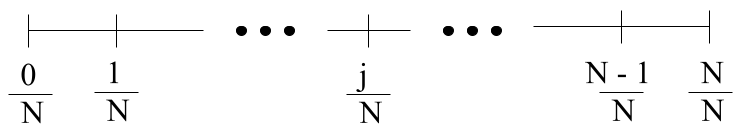
\includegraphics[width=2in]{media/discrete_interval.png}	
		\end{figure}
		\item Choose a finite timestep $k>0$
		\item Let $h=1/N$ and approximate samples of the function: \begin{equation*}
		u_j^n:\approx u(jh,nk)\quad j=0,\ldots,N,\quad n=0,1,\ldots
	\end{equation*}
	\end{itemize}
	
	Discretization of the operators:
	\begin{columns}	
		\begin{column}{.45\paperwidth}
			\begin{equation*}
				\partial_t u_j^n:=\frac{u_j^{n+1}-u_j^n}{k}
			\end{equation*}	
		\end{column}

		\begin{column}{.45\paperwidth}
			\begin{equation}
				\Delta^hu_j^n:=\frac{u_{j+1}^n-2u_j^n+u_{j-1}^n}{h^2}
			\end{equation}
		\end{column}

	\end{columns}

\end{frame}

\begin{frame}{Our Difference Schemes}

	Forward Euler/ central difference schemes for the Heat, Allen-Cahn, and Cahn-Hilliard equations:

	\begin{align}
		\frac{u_j^{n+1}-u_j^n}{k}&=D\Delta^hu_j^n\tag{Heat}\label{eq_HE_DS}\\
		\frac{u_j^{n+1}-u_j^n}{k}&=\gamma\Delta^h u_j^n+\phi(u_j^n)\tag{AC}\label{eq_AC_DS}\\
		\frac{u_j^{n+1}-u_j^n}{k}&=M[\Delta^h(\phi(u_j^n))-\gamma\Delta^h(\Delta^h u_j^n)]\tag{CH}{\label{eq_CH_DS}}
	\end{align}

	Set the gradient-scaling constants $M,D$ to 1

\end{frame}

\begin{frame}{Difference Scheme Stability}

	For the difference scheme solution $u_j^n$, let 
	\begin{equation*}
		u_j^n=\sum_{m=0}^{N-1}\alpha_m^n~\e^{2\pi\i \frac{mj}{N}}
	\end{equation*}
	This form of DFT is consistent with the 1-periodic boundary conditions

	\vspace{10 pt}

	The numerical solution is said to be stable if 
	\begin{equation*}
		|\alpha_m^{n+1}|\le|\alpha_m^n|,\quad\text{for all }0\le m< N
	\end{equation*}

	\vspace{10 pt}
	\begin{columns} % TITLE
		
		\begin{column}{.45\paperwidth}
			\centering
			\small
			Stable: $k=.0012<k_\text{crit}$
			\vspace{-10 pt}
			\begin{figure}
				\centering
				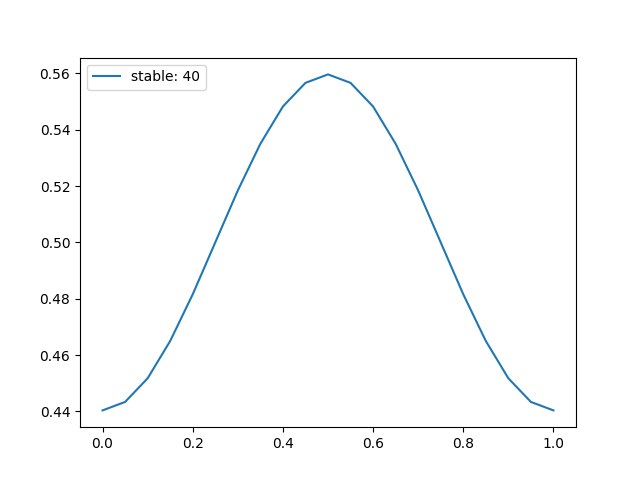
\includegraphics[width = .3\paperwidth]{media/stable.png}	
			\end{figure}	
		\end{column}

		\begin{column}{.45\paperwidth}
			\centering
			\small
			Unstable: $k=.0013>k_\text{crit}$
			\vspace{-10pt}
			\begin{figure}
				\centering
				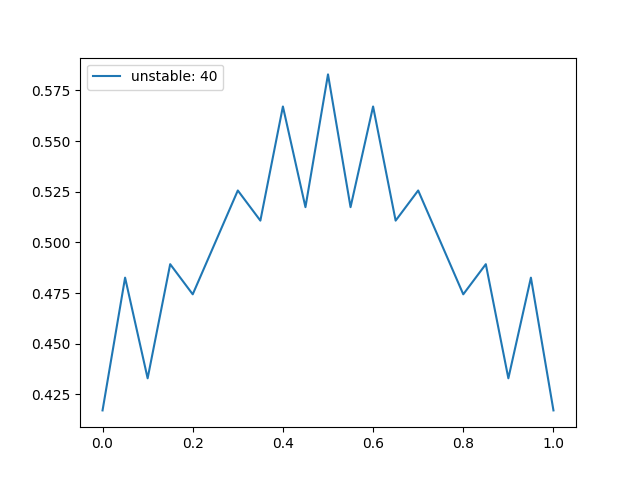
\includegraphics[width = .3\paperwidth]{media/unstable.png}
			\end{figure}
		\end{column}

	\end{columns}

\end{frame}

\begin{frame}{Heat Forward Difference Scheme Stability}
	
	Differentiation in space domain is multiplication in Fourier domain:\begin{align*}
		\Delta^{h}u_{j}^{n}&=\frac{1}{h^2} \sum_{m=0}^{N-1}\alpha_{m}^{n}~\left(\e^{2\pi \i \frac{m(j + 1)}{N}}-2\e^{2\pi\i\frac{mj}{N}}+\e^{2\pi\i\frac{m(j-1)}{N}}\right)\\
		&=\sum_{m=0}^{N-1}\alpha_m^n\underbrace{\frac{1}{h^2}\left( \e^{2\pi\i\frac{m}{N}}+\e^{-2\pi\i\frac{m}{N}}-2 \right)}_{:=\lambda_m}~\e^{2\pi\i\frac{mj}{N}}\\
		&=\sum_{m=0}^{N-1}\lambda_m\alpha_m^n~\e^{2\pi\i\frac{mj}{N}}\\
		\lambda_m&=-\frac{1}{h^2}\left( 2\cos\left( 2\pi\i\frac{m}{N}\right)-2 \right)=-\frac{4}{h^2}\sin^2\left(\pi \frac{m}{N}\right)\tag{Amplification Factor}
	\end{align*}

\end{frame}

\begin{frame}{Heat Forward Difference Scheme Stability}

	Difference scheme in Fourier space: 
	\begin{equation*}
		u_j^{n+1}=u_j^n+k\Delta^hu_j^n\to \alpha_m^{n+1}=\alpha^n_m+k\lambda_m\alpha_m^n=(1+k\lambda_m)\alpha_m^n	
	\end{equation*}

	Stability condition becomes: 
	\begin{equation*}
		\abs{1-\frac{4k}{h^2}\underbrace{\sin^2\left( \pi\frac{m}{N} \right)}_{\ge0}}\le1\iff \frac{4k}{h^2}\underbrace{\sin^2\pi\frac{m}{N}}_{\le1}\le2,\quad m=0,\ldots,N
	\end{equation*}
	Holds when:
	\begin{equation*}
		k\le k_\text{crit}:= \frac{h^2}{2}
	\end{equation*}
	
\end{frame}

\begin{frame}{Stability of Nonlinear Schemes}
	
	Linearized difference scheme stability (about $\pm1$):
	\begin{columns}
		\begin{column}{.45\paperwidth}
			\begin{equation}
				k_{\text{crit}}= \frac{h^2}{h^2+2\gamma}\tag{AC}
			\end{equation}
		\end{column}
		\begin{column}{.45\paperwidth}
			\begin{equation}
				k_{\text{crit}}= \frac{h^4}{4h^2+8\gamma}\tag{CH}
			\end{equation}
		\end{column}
	\end{columns}
	% Due to the equilibrium stability of the differential equation, we postulate that the numerical stabiltiy of the linear analysis reflects the stability of the corresponding nonlinear schemes. Numerical experiments support this ...
	% We expect that the numerical stability of the linear analysis reflects the stability of the corresponding nonlinear schemes, and numerical experiments agree:
	Linear stability analysis reflects stability of nonlinear schemes:

	\vspace{-5 pt}

	\begin{figure} 
		\centering
		% \subfloat[\centering Stable: $k=.11$]{{\animategraphics[width = 4cm, every = 1, loop, autoplay]{2}{media/stability/stable-}{0}{19}} }
		% \qquad
		% \subfloat[\centering Unstable: $k=.12$]{{\animategraphics[width = 4cm, every = 1, loop, autoplay]{1}{media/stability/unstable-}{0}{99}}}

		\animategraphics[width=9cm, every = 1]{1}{media/stability/stability-}{0}{26}
		\\ Numerical results of nonlinear Allen-Cahn equation difference scheme (\ref{eq_AC_DS}) at (left) and above (right) the critical timestep $k_\text{crit}=.11$ for parameters $h=.005,\gamma=.0001$
	\end{figure}
	
\end{frame}

\section{Results}

\begin{frame}{LAMMPS Simulation of Argon Diffusion}

	
	% https://pubs.aip.org/aip/jcp/article/111/20/9352/183481/Lennard-Jones-as-a-model-for-argon-and-test-of

	\begin{columns}

		\begin{column}{.33\paperwidth}
		
			Parameter Values:
			\begin{align*}
				\epsilon &= .24979~\text{kcal/mol}\\
				\sigma&=3.4~\text{\r{A}}\\
				N_A&=700\\
				m&=39.948~\text{g/mol}\\
				T&=300.00~\text{K}\\
				P&=1.14~\text{atm}
			\end{align*}
			\vspace{-10pt}

		\end{column}

		\begin{column}{.62\paperwidth}

			\vspace{-12pt}
			\begin{figure}
				\centering
				\animategraphics[width = .59\paperwidth, every = 1, loop, autoplay]{6}{media/particle_diff/part_diff-}{0}{99}
				
				
			\end{figure}
		\end{column}

	\end{columns}
	
\end{frame}

\begin{frame}{Fitted Difference Results}
	
	\begin{columns}
		
		\begin{column}{.3\paperwidth}

			\centering
			$N=20$

			\begin{figure}

				\animategraphics[width = .3\paperwidth, every = 1]{6}{media/comp/comp20-}{0}{50}
				
			\end{figure}
			
		\end{column}

		\begin{column}{.3\paperwidth}

			\centering
			$N=50$
			
			\begin{figure}

				\animategraphics[width = .3\paperwidth, every = 5]{6}{media/comp/comp50-}{0}{246}
				
			\end{figure}
			
		\end{column}

		\begin{column}{.3\paperwidth}

			\centering
			$N=100$
			
			\begin{figure}

				\animategraphics[width = .3\paperwidth, every = 6]{6}{media/comp/comp100-}{0}{289}
				
			\end{figure}
	
			
		\end{column}
	\end{columns}
	
\end{frame}

\begin{frame}{LAMMPS Simulation of Phase Separation}

	\begin{columns}

		\begin{column}{.33\paperwidth}
		
			Parameter Values:
			\begin{align*}
				\epsilon_{AA} &=\epsilon_{BB} =3.0\\
				\epsilon_{AB}&=1.0\\
				\sigma_*&=1\\
				N_A=N_B&=15000\\
			\end{align*}

		\end{column}

		\begin{column}{.62\paperwidth}

			\vspace{-12pt}
			\begin{figure}
				\centering
				\animategraphics[width = .53\paperwidth, every = 1, loop, autoplay]{15}{media/MD_phase/phase-}{0}{249}
			\end{figure}
		\end{column}

	\end{columns}	

\end{frame}

\begin{frame}{Next Steps}

	\begin{itemize}
		\item Fit the phase separation simulation to the Allen-Cahn and Cahn-Hilliard difference schemes
		\item Look at cost functions for quantitative comparison of the results
	\end{itemize}

	\begin{figure}
		\animategraphics[width = .5\paperwidth, every = 1, loop, autoplay]{5}{media/AC_sep/AC_sep-}{0}{199}
	\end{figure}
	
\end{frame}

\section*{}

\begin{frame}
	\vfill
	\centering
	\begin{beamercolorbox}[sep=8pt,center,shadow=true,rounded=true]{title}
	\usebeamerfont{title}Questions?
	\end{beamercolorbox}
	\vfill
\end{frame}

\end{document}